\documentclass[10pt,a4paper]{article}
\usepackage[margin=18mm,includeheadfoot]{geometry}
\usepackage{fontspec}
\setmainfont{Noto Serif}
\setsansfont{Noto Sans}
\setmonofont{Noto Sans Mono}
\usepackage{amsmath,amssymb,amsthm,mathtools}
\usepackage{graphicx}
\setkeys{Gin}{keepaspectratio}
\usepackage{booktabs,longtable,array,tabularx}
\usepackage{microtype}
\usepackage{enumitem}
\usepackage{xcolor}
\usepackage{hyperref}
\usepackage{bookmark}
\usepackage{fancyvrb}
\usepackage{fvextra}
\usepackage{upquote}
\usepackage{csquotes}
\usepackage{caption}
\usepackage{float}
\usepackage{fancyhdr}
\usepackage{lastpage}
\usepackage{titlesec}
\usepackage{setspace}
\usepackage{etoolbox}
\usepackage{url}
\usepackage{multirow}
\usepackage{makecell}
\hypersetup{colorlinks=true,linkcolor=black,citecolor=black,urlcolor=blue,pdfauthor={Anonymous submission draft},pdftitle={Phase
Erasure Can Hide Agreement-Violation Witnesses in Certificate-Driven
Locking BFT Protocols}}
\setlist{nosep,leftmargin=*}
\setlength{\parindent}{1em}
\setlength{\parskip}{0.25em}
\setlength{\emergencystretch}{2em}
\captionsetup{font=small,labelfont=bf}
\titleformat{\section}{\large\bfseries}{}{0em}{}
\titleformat{\subsection}{\normalsize\bfseries}{}{0em}{}
\titleformat{\subsubsection}{\normalsize\itshape}{}{0em}{}
\titlespacing*{\section}{0pt}{1.0em}{0.35em}
\titlespacing*{\subsection}{0pt}{0.8em}{0.25em}
\titlespacing*{\subsubsection}{0pt}{0.65em}{0.2em}
\newtheorem{theorem}{Theorem}
\newtheorem{lemma}{Lemma}
\newtheorem{proposition}{Proposition}
\newtheorem{definition}{Definition}
\newcommand{\UnsafeObs}{\mathsf{UnsafeObs}}
\newcommand{\tightlist}{\setlength{\itemsep}{0pt}\setlength{\parskip}{0pt}}
\providecommand{\pandocbounded}[1]{#1}
\NewDocumentCommand\citeproctext{}{}
\NewDocumentCommand\citeproc{mm}{%
  \begingroup\def\citeproctext{#2}\cite{#1}\endgroup}
\makeatletter
\let\@cite@ofmt\@firstofone
\def\@biblabel#1{}
\def\@cite#1#2{{#1\if@tempswa , #2\fi}}
\makeatother
\newlength{\cslhangindent}
\setlength{\cslhangindent}{1.5em}
\newlength{\csllabelwidth}
\setlength{\csllabelwidth}{3em}
\newenvironment{CSLReferences}[2]
 {\begin{list}{}{%
  \setlength{\itemindent}{0pt}
  \setlength{\leftmargin}{0pt}
  \setlength{\parsep}{0pt}
  \ifodd #1
   \setlength{\leftmargin}{\cslhangindent}
   \setlength{\itemindent}{-1\cslhangindent}
  \fi
  \setlength{\itemsep}{#2\baselineskip}}}
 {\end{list}}
\newcommand{\CSLBlock}[1]{\hfill\break\parbox[t]{\linewidth}{\strut\ignorespaces#1\strut}}
\newcommand{\CSLLeftMargin}[1]{\parbox[t]{\csllabelwidth}{\strut#1\strut}}
\newcommand{\CSLRightInline}[1]{\parbox[t]{\dimexpr\linewidth-\csllabelwidth\relax}{\strut#1\strut}}
\newcommand{\CSLIndent}[1]{\hspace{\cslhangindent}#1}
\pagestyle{fancy}
\fancyhf{}
\lhead{Anonymous Gate 8′ submission draft}
\rhead{\thepage/\pageref{LastPage}}
\renewcommand{\headrulewidth}{0.2pt}
\begin{document}

\begin{titlepage}
\centering
\vspace*{22mm}
{\LARGE\bfseries Phase Erasure Can Hide Agreement-Violation Witnesses in
Certificate-Driven Locking BFT Protocols\par}
\vspace{14mm}
{\large Anonymous submission draft\par}
\vspace{8mm}
{\small Evidence cut-off: 17 August 2026\par}
\vfill
\begin{minipage}{0.88\textwidth}
\textbf{Abstract.}
Fault-injection frameworks for Byzantine fault-tolerant protocols expose
different amounts of control over message delivery: some choose a
partition or directed communication graph for an entire view, while
others distinguish message phases, individual instances, or replay. A
richer scheduler trivially generates more executions, but it is unclear
when that additional authority changes the set of safety-relevant
observations rather than merely producing redundant traces.

We study closure from phase-specific delivery to one type-uniform
directed endpoint graph for finite certificate-driven locking schemas.
First, we give a relational sufficient condition under which
closure-added messages preserve an unsafe observation. We then identify
its locking boundary: repair evidence added by type erasure can disable
the unique honest participant shared by two conflicting quorums. For
every \(f\geq1\), with \(n=3f+1\) and \(q=2f+1\), we construct an
explicit schema in which phase-specific delivery forms both conflicting
certificates, whereas both directed-edge choices remain safe. We derive
an exact seven-premise characterization of this construction and
separately prove that exact replay is observationally erasable under
stable-key idempotence.

The obligations are independently re-encoded as Z3 CHC/SMT queries,
cross-checked with exact Go big-integer arithmetic, and reproduced in
two bounded locking kernels plus a fuller two-round Go event loop and an
independent Python mirror. The work establishes an explicit
safety-observation boundary; it does not claim universal incompleteness
of graph-based schedulers, a production-client vulnerability, or a
liveness result.
\end{minipage}
\vfill
{\small Best student paper eligibility: not specified in the research brief.\par}
{\small This cover page is a working OPODIS-style submission cover, not final metadata.\par}
\end{titlepage}

\begin{center}
{\LARGE\bfseries Phase Erasure Can Hide Agreement-Violation Witnesses in
Certificate-Driven Locking BFT Protocols\par}
\vspace{1.0em}
{\large Anonymous submission draft\par}
\end{center}

\begin{abstract}
Fault-injection frameworks for Byzantine fault-tolerant protocols expose
different amounts of control over message delivery: some choose a
partition or directed communication graph for an entire view, while
others distinguish message phases, individual instances, or replay. A
richer scheduler trivially generates more executions, but it is unclear
when that additional authority changes the set of safety-relevant
observations rather than merely producing redundant traces.

We study closure from phase-specific delivery to one type-uniform
directed endpoint graph for finite certificate-driven locking schemas.
First, we give a relational sufficient condition under which
closure-added messages preserve an unsafe observation. We then identify
its locking boundary: repair evidence added by type erasure can disable
the unique honest participant shared by two conflicting quorums. For
every \(f\geq1\), with \(n=3f+1\) and \(q=2f+1\), we construct an
explicit schema in which phase-specific delivery forms both conflicting
certificates, whereas both directed-edge choices remain safe. We derive
an exact seven-premise characterization of this construction and
separately prove that exact replay is observationally erasable under
stable-key idempotence.

The obligations are independently re-encoded as Z3 CHC/SMT queries,
cross-checked with exact Go big-integer arithmetic, and reproduced in
two bounded locking kernels plus a fuller two-round Go event loop and an
independent Python mirror. The work establishes an explicit
safety-observation boundary; it does not claim universal incompleteness
of graph-based schedulers, a production-client vulnerability, or a
liveness result.
\end{abstract}

\noindent\textbf{Keywords:} Byzantine fault tolerance, consensus
testing, scheduler expressiveness, communication closure, quorum
certificates, formal methods, reproducibility
\vspace{0.6em}

\section{1. Introduction}\label{introduction}

Byzantine fault-tolerant (BFT) consensus protocols are tested under
adversarial message schedules because the same protocol code can exhibit
materially different behavior when messages are dropped, delayed,
reordered, duplicated, or selectively delivered. Testing frameworks
expose this adversarial authority through a \emph{scheduler grammar}: a
language for saying which communication actions are permitted in each
execution. Twins uses replicas with a shared identity and round-indexed
communication partitions to realize equivocation-like scenarios without
a hand-written malicious implementation (Bano et al. 2022).
Communication-closure testing reduces asynchronous executions to
controlled round-based schedules for a suitable class of consensus
implementations (Drăgoi et al. 2020). ByzzFuzz adds randomized message
mutations and partitions (Winter et al. 2023), Netrix offers
programmer-guided filters and monitors (Drăgoi, Nagendra, and Srivas
2024), and ByzzBench provides common infrastructure for comparing
testing algorithms (Neto and Ozkan 2025).

These systems differ in more than search strategy. A partition schedule
makes one symmetric connectivity choice for a view. A directed schedule
distinguishes sender--receiver orientation. A phase-specific schedule
can separate two messages that share the same endpoint pair but serve
different protocol roles. A per-instance scheduler can additionally
distinguish individual messages and delivery order. A replay-capable
scheduler may deliver the same logical signed action more than once.

The corresponding raw execution languages are ordered almost by
definition: every partition schedule can be represented by a directed
graph, every phase-specific graph can be represented by per-instance
decisions, and so on. That inclusion is not the scientific question. Two
grammars may generate different internal traces while exposing exactly
the same agreement violations. Conversely, a coarser grammar may be
forced to deliver an additional valid message whose protocol effect
\emph{repairs} the unsafe execution. We therefore study a
property-preserving closure problem:

\begin{quote}
\textbf{Central question.} When does erasing message-phase distinctions
to one type-uniform directed endpoint graph preserve every finite
agreement-violation observation, and when can the messages added by that
closure destroy the witness?
\end{quote}

The mechanism is non-monotone locking repair. Suppose closure inserts
only transitions that are increasing in a preorder under which the
unsafe set is upward closed. Then unsafety survives. A repair or
terminal certificate in a locking protocol need not satisfy that
premise: receiving it may strengthen a lock, cause an irreversible
decision, or otherwise remove a validator from a future conflicting
quorum. If that validator is the unique honest pivot shared by two
quorums, closure can change an unsafe trace into a safe one even though
it only \emph{adds} deliveries.

This distinction matters for the interpretation of fault-injection
results. The richer scheduler is not automatically better merely because
it generates more traces, and the coarser scheduler is not automatically
safety-complete merely because it represents partitions or arbitrary
directed graphs. What matters is whether a closure between grammars
preserves the selected safety observation for the protocol class under
study.

\subsection{1.1 Contributions}\label{contributions}

This paper makes three narrow contributions.

\begin{enumerate}
\def\labelenumi{\arabic{enumi}.}
\item
  \textbf{Relational closure lifting.} We state and prove a sufficient
  condition under which inserting the messages required by a coarser
  scheduler preserves a finite unsafe observation. The theorem exposes
  the exact local obligations: inserted actions must be increasing under
  a preorder, retained actions must forward-simulate it, and the unsafe
  set must be upward closed.
\item
  \textbf{Parametric quorum-pivot separation and exact premise
  boundary.} For every integer \(f\geq1\), with \(n=3f+1\) and quorum
  threshold \(q=2f+1\), we construct a two-branch certificate-driven
  schema in which a phase-specific scheduler can form two conflicting
  certificates, while both choices of the corresponding type-uniform
  directed edge remain safe. The construction isolates a unique honest
  quorum pivot and two differently labelled messages, enabling evidence
  \(E\) and later repair evidence \(R\), on the same edge. For the
  supplied seven-flag operational abstraction, strict separation holds
  exactly when

  \[S_2\land D\land T\land E_d\land X\land(S_1\lor R_q).\]
\item
  \textbf{Replay boundary and executable assurance.} We prove that exact
  replay is observationally erasable when processing is idempotent under
  a stable logical key, and give the complementary counterexample when
  quorum code counts message instances. We validate the scheduler
  separation in two exact locking kernels and in a fuller two-round
  event loop implemented independently in Go and Python. The formal
  obligations are separately encoded as SMT and constrained Horn-clause
  queries with satisfiable damaged controls.
\end{enumerate}

The paper is deliberately not framed as a new testing domain-specific
language. Partition scenarios, message filters, delay, reordering,
replay, mutation-based BFT testing, and benchmark infrastructure are
prior art (Bano et al. 2022; Winter et al. 2023; Drăgoi, Nagendra, and
Srivas 2024; Neto and Ozkan 2025). The contribution is the effect of one
closure transformation on the \emph{unsafe-observation language}.

\subsection{1.2 Scope and nonclaims}\label{scope-and-nonclaims}

The results concern finite agreement observations of explicit
certificate-driven schemas. They are not a universal incompleteness
theorem for partition or directed schedulers. They do not establish a
vulnerability in HotStuff, Tendermint, CometBFT, or any deployed client.
They do not address liveness or unbounded partial synchrony, and they do
not estimate the prevalence or discovery probability of real bugs. The
production specifications and source snapshots in the artifact are used
to discipline terminology and implementation assumptions, not as
evidence of a production defect.

\section{2. Model and problem
statement}\label{model-and-problem-statement}

\subsection{2.1 Certificate-driven locking
schema}\label{certificate-driven-locking-schema}

A phase-labelled certificate-driven protocol is a tuple

\[
P=(N,V,\Lambda,S,M,\delta,\mathsf{emit},O),
\]

where \(N\) is a finite set of logical validator identities, \(V\) is an
ordered set of views or rounds, \(\Lambda\) is a finite set of phases,
\(S=\prod_{i\in N}S_i\) is the product of local states, and \(M\) is a
set of authenticated messages. For a correct validator \(i\), the
deterministic handler

\[
\delta_i:S_i\times M\rightarrow S_i\times M^{*}
\]

updates local state and emits a finite sequence of messages. The
function \(\mathsf{emit}\) abstracts phase barriers or message
production that is not triggered by one incoming message. The
observation function \(O:S\rightarrow\Omega\) selects protocol-relevant
terminal data.

Every controlled message has at least the fields

\[
(sender,receiver,view,phase,kind,payload,replay\_key,contribution\_key).
\]

The \texttt{replay\_key} identifies one exact signed protocol action.
Re-delivery of that action has the same key. The
\texttt{contribution\_key} identifies the logical voting slot whose
weight may be counted at most once, normally a tuple such as height,
round, vote phase, and validator identity. Two equivocations may have
different replay keys while competing for the same contribution key.

The schema abstracts signatures by assuming that a scheduler cannot
forge a message attributed to a correct identity and that certificate
signer sets are explicit. The central separation does not depend on a
particular signature scheme. Byzantine identities may contribute to
conflicting certificates, as usual in a Byzantine fault model (Lamport,
Shostak, and Pease 1982).

A \emph{lock} is persistent protocol state restricting future support.
The schema does not require one universal lock rule; the separation only
requires that a later repair or terminal message can remove one honest
validator from a conflicting branch. This may occur by strengthening a
lock, finalizing a value, or setting another state predicate that blocks
the relevant contribution.

\subsection{2.2 Safety observation}\label{safety-observation}

Let \(H\subseteq N\) be the correct validators. For agreement, the
terminal observation is

\[
O_s(s)=(decision_i)_{i\in H}.
\]

A state is unsafe when two correct identities have distinct non-null
decisions:

\[
\mathsf{Unsafe}(s)\equiv \exists i,j\in H.\ decision_i\neq\bot\land decision_j\neq\bot\land decision_i\neq decision_j.
\]

The observation intentionally excludes internal logs, counters, and
transient scheduling state unless they change a protocol-visible
transition. This prevents a raw trace difference from being mistaken for
a safety separation.

\subsection{2.3 Scheduler grammars}\label{scheduler-grammars}

We compare six grammars. Within a view or round:

\begin{longtable}[]{@{}
  >{\raggedright\arraybackslash}p{(\columnwidth - 4\tabcolsep) * \real{0.3333}}
  >{\raggedright\arraybackslash}p{(\columnwidth - 4\tabcolsep) * \real{0.3333}}
  >{\raggedright\arraybackslash}p{(\columnwidth - 4\tabcolsep) * \real{0.3333}}@{}}
\toprule\noalign{}
\begin{minipage}[b]{\linewidth}\raggedright
Grammar
\end{minipage} & \begin{minipage}[b]{\linewidth}\raggedright
Control authority
\end{minipage} & \begin{minipage}[b]{\linewidth}\raggedright
Direct extension
\end{minipage} \\
\midrule\noalign{}
\endhead
\bottomrule\noalign{}
\endlastfoot
\(G_P\) & one symmetric partition relation & \(G_D\): relax symmetry \\
\(G_D\) & one directed endpoint graph, uniform over controlled phases &
\(G_T\): retain phase labels; \(G_{D1}\): add bounded terminal delay \\
\(G_{D1}\) & \(G_D\) plus one-view deferral of terminal evidence &
separate temporal branch \\
\(G_T\) & one directed graph per phase or message type & \(G_M\): retain
instance identity and order \\
\(G_M\) & independent delivery/order per message instance & \(G_R\):
permit replay \\
\(G_R\) & \(G_M\) plus bounded replay of stable logical messages &
--- \\
\end{longtable}

The constructive embeddings used by the checkers are

\[
G_P\subseteq G_D\subseteq G_T\subseteq G_M\subseteq G_R,
\qquad G_D\subseteq G_{D1}.
\]

No inclusion is asserted between \(G_{D1}\) and \(G_T\): one adds
temporal control, whereas the other retains phase labels. Round-based
directed communication graphs are established models in the
message-adversary literature (Charron-Bost and Schiper 2009; Winkler,
Schmid, and Moses 2020). Here they are not proposed as a new model; they
form the coarser target of the closure we analyze.

\begin{figure}
\centering
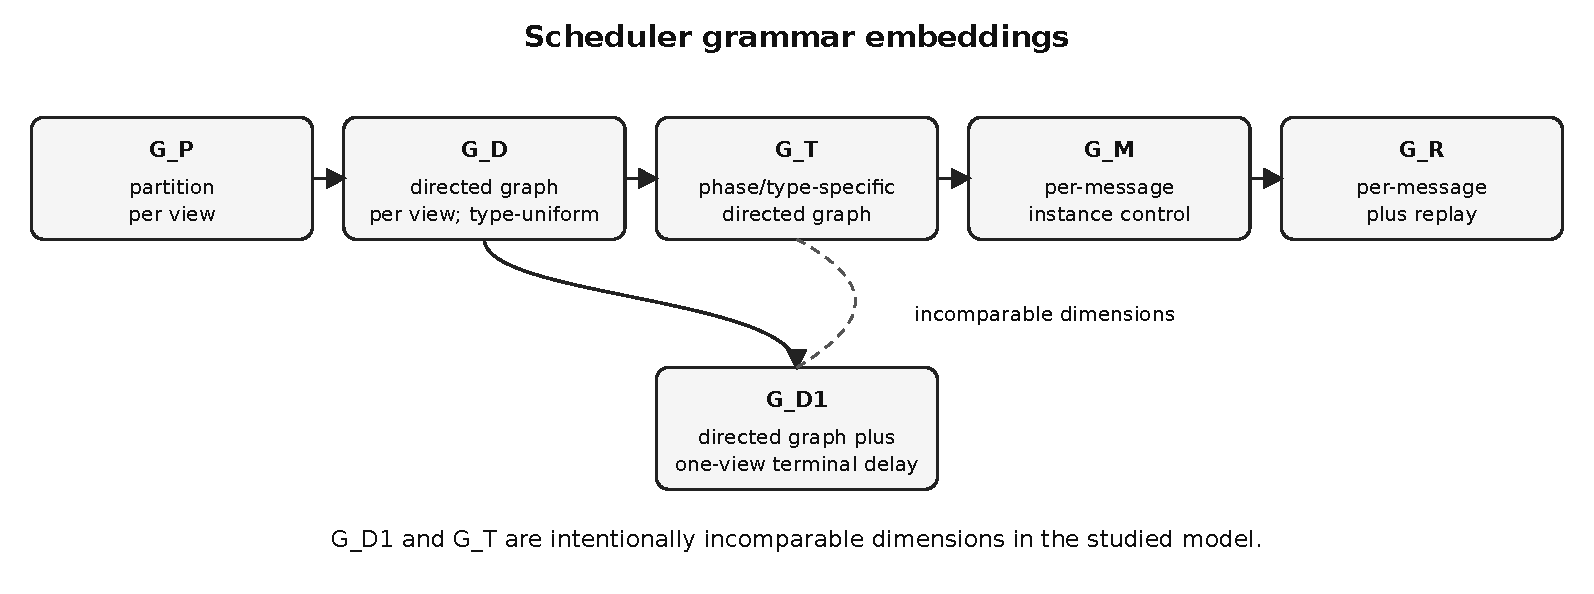
\includegraphics[width=0.92\textwidth,height=\textheight]{figures/figure1_scheduler_grammar.pdf}
\caption{Scheduler grammar embeddings. The bounded-delay branch is
intentionally not ordered against the phase-specific
branch.}\label{fig:grammar}
\end{figure}

\subsection{2.4 Execution and observation
languages}\label{execution-and-observation-languages}

For a protocol \(P\), scheduler grammar \(G\), and bounded domain \(B\),
let \(L_G(P,B)\) be the set of admissible executions. The bounded domain
fixes such quantities as the finite participant set, view horizon,
values, and controlled message production. Define

\[
\mathsf{UnsafeObs}_G(P,B)=
\{O_s(\tau)\mid \tau\in L_G(P,B)\land \mathsf{Unsafe}(O_s(\tau))\}.
\]

Raw language inclusion \(L_{G_1}\subseteq L_{G_2}\) does not imply a
strict inclusion of unsafe observations. A bounded experimental
separation requires an observation reachable under the stronger grammar
and absent from the \emph{complete} weaker language in the stated
domain. A symbolic separation, by contrast, gives a family of schemas
and proves the distinction independent of finite enumeration.

\subsection{2.5 Closure operators}\label{closure-operators}

Three closures are relevant.

\textbf{Phase/type erasure \(C_{type}\).} Starting from a \(G_T\)
schedule, retain every directed endpoint edge used in a view and admit
every controlled phase on that edge. The closure erases phase
selectivity but does not add reverse edges.

\textbf{Terminal-time erasure \(C_{time}\).} Starting from a \(G_{D1}\)
schedule, deliver admitted terminal evidence immediately rather than in
the next view.

\textbf{Replay erasure \(C_{dup}\).} Starting from a \(G_R\) trace,
retain the first delivery of each replay key and delete later identical
deliveries. Distinct signed actions and equivocations remain.

The rest of the paper characterizes when these closures preserve the
selected finite safety observation.

\section{3. Relational closure
lifting}\label{relational-closure-lifting}

\subsection{3.1 Merged traces}\label{merged-traces}

Let \(\tau=a_1\ldots a_k\) be an original finite execution. A closure
trace \(C(\tau)\) is a merged sequence that retains every original
action in the same relative order and inserts additional actions
required by the coarser grammar. For phase erasure, an inserted action
is typically the delivery of a different phase label on an endpoint edge
that the original trace used for some other label.

Let \(\mathcal{S}\) be the protocol-relevant state space and
\(R\subseteq\mathcal{S}\times\mathcal{S}\) a preorder. Intuitively,
\(R(s,t)\) means that \(t\) contains at least the safety-relevant
progress represented by \(s\). This interpretation is deliberately
conditional: a protocol instance must supply a meaningful relation, and
a repair transition may make such a relation impossible.

\subsection{3.2 Sufficient conditions}\label{sufficient-conditions}

We use four obligations.

\begin{enumerate}
\def\labelenumi{\arabic{enumi}.}
\tightlist
\item
  \textbf{Initial relation.} The original and closure executions start
  in related states.
\item
  \textbf{Increasing insertion.} For every closure-added action \(b\),
  if \(b\) maps \(t\) to \(t'\), then \(R(t,t')\).
\item
  \textbf{Forward simulation of retained actions.} If \(R(s,t)\) and an
  original action \(a\) maps \(s\) to \(s'\), then the corresponding
  retained action maps \(t\) to some \(t'\) such that \(R(s',t')\).
\item
  \textbf{Upward-closed unsafety.} If \(\mathsf{Unsafe}(s)\) and
  \(R(s,t)\), then \(\mathsf{Unsafe}(t)\).
\end{enumerate}

\subsubsection{Theorem 1 (Relational closure lifting;
T2)}\label{theorem-1-relational-closure-lifting-t2}

Let \(\tau\) be a finite execution ending in an unsafe state. Let
\(C(\tau)\) preserve the order of the original actions and insert only
closure-added actions. If a preorder \(R\) satisfies the four
obligations above, then the terminal state of \(C(\tau)\) is unsafe.

\subsubsection{Proof}\label{proof}

Traverse the merged trace while relating the state after the original
actions consumed so far to the state after the corresponding merged
prefix. Initially the relation holds by premise 1. When the next merged
action is inserted, the original side does not move; increasing
insertion and transitivity preserve the relation. When the next merged
action is retained from \(\tau\), both sides advance and forward
simulation preserves the relation. Induction over the finite merged
trace therefore relates the unsafe terminal state of \(\tau\) to the
terminal state of \(C(\tau)\). Upward closure of unsafety yields the
result. \(\square\)

If \(R\) additionally preserves the complete selected observation in
both directions, the same argument yields observation equality rather
than only preservation of unsafety. The weaker theorem is more useful
here because the closure may legitimately change non-safety state.

\subsection{3.3 Why the theorem is not
tautological}\label{why-the-theorem-is-not-tautological}

The theorem does not assume that every added message is harmless. That
is precisely the per-instance obligation. An inserted message may
violate increasingness for any preorder that preserves future quorum
participation. For example, a terminal certificate delivered to a pivot
may cause an irreversible decision and suppress the pivot's later vote
for a conflicting value. The closure state then contains \emph{more
received evidence} but \emph{fewer available future actions}. A naïve
subset order on received messages is therefore insufficient.

The parametric construction in the next section is a failed-premise
boundary of Theorem 1. It demonstrates that the missing monotonicity is
not merely a formal technicality: it determines whether an
agreement-violation witness exists.

\section{4. Parametric quorum-pivot
separation}\label{parametric-quorum-pivot-separation}

\subsection{4.1 Construction}\label{construction}

Fix an arbitrary integer \(f\geq1\). Let

\[
n=3f+1,\qquad q=2f+1.
\]

Partition the validator identities into four disjoint sets:

\begin{itemize}
\tightlist
\item
  \(B\), containing \(f\) Byzantine identities;
\item
  \(A\), containing \(f\) correct identities supporting value \(0\);
\item
  \(C\), containing \(f\) correct identities supporting value \(1\);
\item
  a single correct pivot \(p\).
\end{itemize}

Define the conflicting supports

\[
Q_0=B\cup A\cup\{p\},\qquad Q_1=B\cup C\cup\{p\}.
\]

Both sets have size \(q\). Their intersection is \(B\cup\{p\}\), so
\(p\) is their only correct shared identity. Without \(p\), each branch
has support \(2f=q-1\).

The schema has two differently labelled messages on the same
sender-to-pivot edge:

\begin{itemize}
\tightlist
\item
  enabling evidence \(E\), which makes \(p\) contribute to the first
  branch and, under the controlled defective transition, leaves \(p\)
  eligible for the second branch;
\item
  later repair or terminal evidence \(R\), which, if delivered before
  the second quorum opportunity, disables the conflicting contribution
  of \(p\).
\end{itemize}

The fixed supporters in \(B\cup A\) and \(B\cup C\) contribute to their
respective branches, and no other validator can replace \(p\). The
construction requires only two conflicting certificate opportunities; it
does not assume a complete implementation of one named protocol.

\begin{figure}
\centering
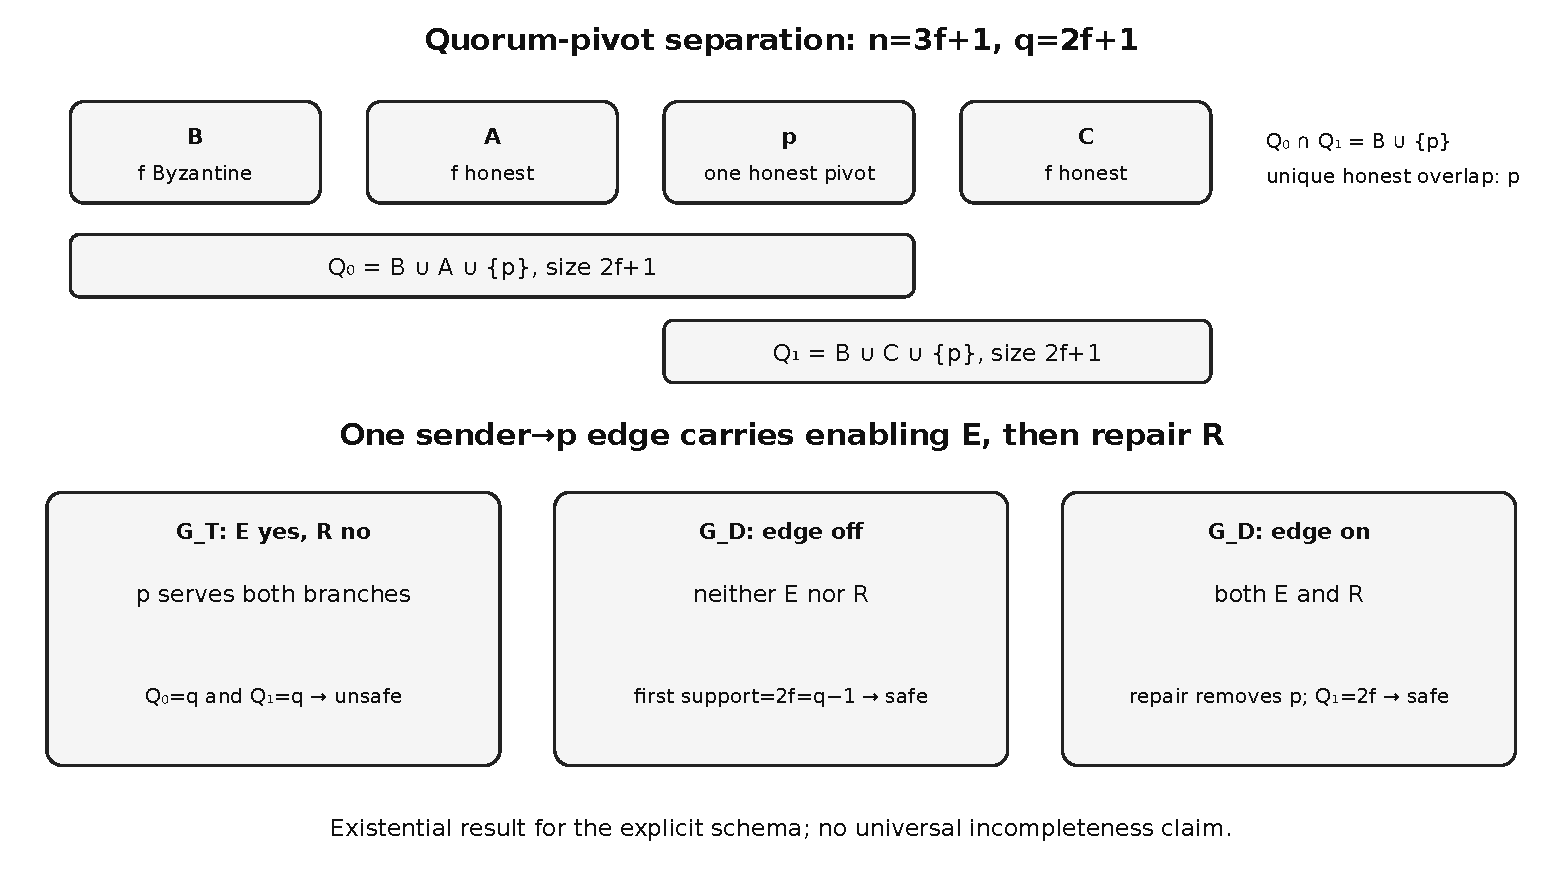
\includegraphics[width=0.96\textwidth,height=\textheight]{figures/figure2_quorum_pivot.pdf}
\caption{Quorum-pivot construction. Phase-specific delivery admits
enabling evidence \(E\) while withholding repair evidence \(R\) on the
same edge. Type erasure couples the two labels.}\label{fig:pivot}
\end{figure}

\subsection{4.2 Phase-specific witness}\label{phase-specific-witness}

A \(G_T\) schedule may admit \(E\) and omit \(R\) on the shared endpoint
edge. The first branch then has

\[
|B|+|A|+1=f+f+1=2f+1=q
\]

supporters. Because the defective transition does not retain the
intended safety constraint and \(R\) is absent, the pivot remains
eligible for the second branch, which likewise has

\[
|B|+|C|+1=q
\]

supporters. Two conflicting certificates and an agreement-violating
terminal observation are reachable.

\subsection{4.3 Type-uniform directed
closure}\label{type-uniform-directed-closure}

A \(G_D\) schedule has one Boolean choice for the endpoint edge carrying
both \(E\) and \(R\).

\textbf{Edge absent.} Neither message reaches \(p\). In the symmetric
core construction, the first branch remains at \(|B|+|A|=2f=q-1\), so
the pair of conflicting certificates cannot form.

\textbf{Edge present.} Both messages reach \(p\). The first branch may
reach quorum, but \(R\) acts before the second certificate opportunity
and disables the pivot. The second branch remains at \(|B|+|C|=2f=q-1\).

These cases exhaust the type-uniform edge choices.

\subsubsection{Theorem 2 (Parametric quorum-pivot separation;
T3)}\label{theorem-2-parametric-quorum-pivot-separation-t3}

For every integer \(f\geq1\), there exists a finite two-branch
certificate-driven schema with \(n=3f+1\) and \(q=2f+1\) such that

\[
\mathsf{UnsafeObs}_{G_D}=\varnothing,
\qquad
\mathsf{UnsafeObs}_{G_T}\neq\varnothing.
\]

\subsubsection{Proof}\label{proof-1}

The phase-specific schedule forms both quorums by the arithmetic above.
Under \(G_D\), the shared edge is absent or present. In the absent case
the first branch is one contribution short; in the present case repair
disables \(p\) and the second branch is one contribution short. Thus
neither \(G_D\) branch produces the conflicting-certificate observation,
whereas \(G_T\) does. \(\square\)

The theorem is symbolic in \(f\). Its universal arithmetic step is not
inferred from sampling. The artifact separately checks the identities
with quantifier-free linear integer arithmetic and with exact Go
\texttt{math/big} calculations for 1,028 positive values, including a
400-digit input, as an implementation-independence regression test.

\subsection{4.4 Interpretation and
scope}\label{interpretation-and-scope}

Theorem 2 is an existential family. It does not state that every
HotStuff-like or Tendermint-like protocol separates \(G_D\) from
\(G_T\). An instantiation must exhibit the relevant phase coupling,
timing, repair effect, shared endpoint edge, and unique honest quorum
pivot. A protocol without such a mechanism may satisfy the closure
theorem of Section 3 or may require a different separation.

The construction also explains why merely comparing raw trace counts
would be misleading. The type-uniform closure delivers \emph{more}
messages than the unsafe phase-specific trace. Those extra messages do
not expose a new violation; they remove the only honest participation
pattern that enabled the second conflicting certificate.

\section{5. Exact premise
characterization}\label{exact-premise-characterization}

The parametric schema deliberately highlights seven Boolean structural
premises. For the operational abstraction in the artifact, they are:

\begin{itemize}
\tightlist
\item
  \(S_1\): the first base support is exactly one below quorum;
\item
  \(S_2\): the second base support is exactly one below quorum;
\item
  \(R_q\): the second use of the pivot requires enabling evidence;
\item
  \(D\): repair disables the pivot;
\item
  \(T\): repair is effective before the second quorum opportunity;
\item
  \(E_d\): enabling and repair share one endpoint edge;
\item
  \(X\): the phase-specific grammar can separate the two labels.
\end{itemize}

The executable model evaluates all \(2^7=128\) assignments, and a
separate Boolean SMT encoding checks equivalence with the closed form.

\subsubsection{Theorem 3 (Exact seven-premise boundary;
T6)}\label{theorem-3-exact-seven-premise-boundary-t6}

For the supplied seven-flag operational construction, strict separation
holds exactly when

\[
S_2\land D\land T\land E_d\land X\land(S_1\lor R_q).
\]

In field order \((S_1,S_2,R_q,D,T,E_d,X)\), the only strict assignments
are

\[
0111111,\quad1101111,\quad1111111.
\]

\subsubsection{Interpretation}\label{interpretation}

Five premises are necessary in every strict assignment of this model:
the second branch must depend on the pivot; repair must disable the
pivot; repair must act in time; the two messages must be coupled by
endpoint erasure; and the stronger grammar must distinguish them.
Neither \(S_1\) nor \(R_q\) is individually necessary, but at least one
is required. Intuitively, the first branch must depend on the enabling
edge either directly through a one-short base or indirectly because the
pivot's later contribution requires the enabling action.

\begin{figure}
\centering
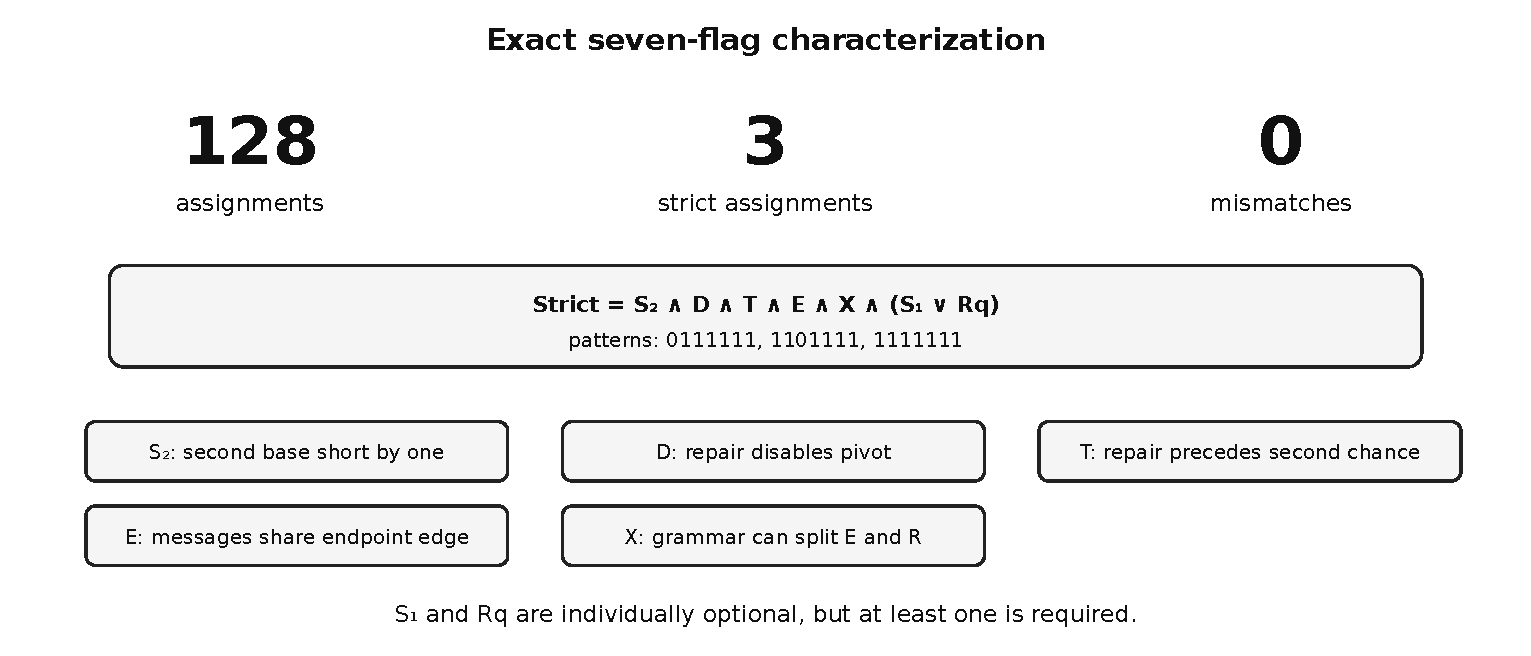
\includegraphics[width=0.92\textwidth,height=\textheight]{figures/figure3_premise_boundary.pdf}
\caption{Exact premise boundary for the supplied Boolean model. Only
three of 128 assignments yield strict separation.}\label{fig:premises}
\end{figure}

\begin{longtable}[]{@{}ll@{}}
\toprule\noalign{}
Item & Exact result \\
\midrule\noalign{}
\endhead
\bottomrule\noalign{}
\endlastfoot
Assignments & 128 \\
Strict assignments & 3 \\
Strict patterns & \texttt{0111111}, \texttt{1101111},
\texttt{1111111} \\
Formula & \(S_2\land D\land T\land E_d\land X\land(S_1\lor R_q)\) \\
Mismatches between executable model and formula & 0 \\
\end{longtable}

Theorem 3 is a characterization of the small operational construction,
not of all certificate-driven protocols. Its purpose is to replace an
informal list of ``likely important'' assumptions with an exact boundary
that can be falsified, ablated, and used as a protocol-mapping
checklist.

\section{6. Replay erasure and its
boundary}\label{replay-erasure-and-its-boundary}

Phase erasure concerns messages with different protocol roles. Replay is
a separate dimension: the same logical signed action may be delivered
repeatedly. A scheduler that allows replay is not necessarily stronger
with respect to state-based safety.

\subsection{6.1 Stable-key idempotence}\label{stable-key-idempotence}

Assign each logical signed message a stable replay key \(\kappa(m)\),
for example

\[
\kappa(m)=(height,round,phase,value,validator).
\]

A second signed value is an equivocation and has a different key. Let
\(\mathsf{dedup}(\tau)\) retain the first occurrence of each replay key
in a finite delivery trace \(\tau\).

Processing is \emph{stable-key idempotent} when every non-first delivery
of a processed key:

\begin{enumerate}
\def\labelenumi{\arabic{enumi}.}
\tightlist
\item
  leaves protocol-relevant state unchanged;
\item
  emits no protocol-relevant output;
\item
  adds no voting power or signer contribution;
\item
  leaves the selected state-based safety observation unchanged; and
\item
  does not affect subsequent protocol-relevant behavior.
\end{enumerate}

\subsubsection{Theorem 4 (Replay erasure;
T1)}\label{theorem-4-replay-erasure-t1}

For every initial state \(s_0\) and finite trace \(\tau\), stable-key
idempotence implies

\[
\delta^{*}(s_0,\tau)=
\delta^{*}(s_0,\mathsf{dedup}(\tau))
\]

on protocol-relevant state. Consequently, quorum status and every
state-based safety observation are equal before and after replay
erasure.

\subsubsection{Proof}\label{proof-2}

Induct on the trace length. The empty trace is immediate. Write
\(\tau=\rho\cdot m\). If \(\kappa(m)\) does not occur in \(\rho\), both
the original and deduplicated executions process \(m\) after equal
protocol-relevant states by the induction hypothesis. If the key already
occurs, deduplication removes \(m\), while the original execution
performs a protocol-relevant stutter and emits no relevant output. The
terminal states remain equal. \(\square\)

\subsection{6.2 Non-idempotent boundary}\label{non-idempotent-boundary}

The assumptions are essential. Suppose a quorum accumulator counts
message instances rather than unique logical contributions. For
threshold three, the sequence

\begin{verbatim}
B, H1, H1
\end{verbatim}

contains only two validator contributions but three message deliveries.
An incorrect instance counter reaches quorum only in the replay-capable
grammar. This is a constructive boundary, not an allegation about a
specific client.

Replay erasure also does not apply when duplicate processing resets
timers, triggers externally visible callbacks, changes resource state
included in the observation, or otherwise modifies subsequent behavior.
Nor does it erase equivocations with different replay keys.

\subsection{6.3 Relationship to scheduler
closure}\label{relationship-to-scheduler-closure}

Theorem 4 gives a case in which additional scheduler authority is
provably redundant for the chosen observation. Theorem 2 gives a case in
which retaining a phase distinction is essential. Together they
illustrate the intended methodology: scheduler grammars should be
compared through property-preserving transformations and explicit
premises, not ranked solely by the number of actions in their API.

\section{7. Executable validation}\label{executable-validation}

The symbolic separation is the central contribution. Executable models
serve three narrower purposes: they test whether the mechanism survives
a less algebraic event semantics, expose implementation confounders, and
provide replayable witnesses. They do not turn a bounded experiment into
a universal protocol theorem.

\subsection{7.1 Exact locking kernels}\label{exact-locking-kernels}

Two dependency-free finite-state kernels instantiate certificate-driven
locking behavior with \(n=4\), \(f=1\), and quorum \(q=3\). Both use one
Byzantine logical identity represented by two physical branches, three
correct identities, binary conflicting values, two rounds, and an
independent agreement oracle.

The first kernel uses generic proposal, vote, intermediate-certificate,
precommit, and commit evidence. The second uses Tendermint-style
vocabulary: proposal, prevote, POLKA, persistent lock and valid-round
state, precommit, and commit. The pinned CometBFT specification and
source snapshot are used only to check that these phase and lock
concepts are natural engineering abstractions (CometBFT Project 2026).
The kernels contain controlled obligation violations, not discovered
production defects.

Across both kernels, the correct baseline remains safe under all tested
scheduler grammars. Controlled mutations show distinct expressiveness
boundaries:

\begin{itemize}
\tightlist
\item
  omitting a lock update or using a wrong justification guard is hidden
  from the type-uniform directed grammar but exposed by phase-specific
  delivery;
\item
  one-view delay of terminal evidence detects some lock-related
  mutations but not a defect requiring discrimination between two
  intermediate quorum-forming phases;
\item
  a duplicate-counting mutation requires replay;
\item
  a receiver-validation omission is a positive control detectable
  already under a partition grammar.
\end{itemize}

These outcomes prevent the checker from being interpreted as a machine
that mechanically declares richer grammars necessary for every defect.

\subsection{7.2 Fuller two-round event
loop}\label{fuller-two-round-event-loop}

The stronger validation route is an explicit event loop with dynamically
generated messages and phases

\begin{verbatim}
PROPOSAL -> PREVOTE -> POLKA -> PRECOMMIT -> COMMIT.
\end{verbatim}

The logical participants are leader \(B\) and correct replicas \(H1\),
\(P\), and \(H3\). Round 0 proposes value \(0\) to \(H1\) and pivot
\(P\); round 1 proposes value \(1\) to \(P\) and \(H3\). Votes are
indexed by unique contribution keys, a POLKA forms after three unique
prevotes, and COMMIT evidence forms after three unique precommits. Locks
persist across rounds, decisions are irreversible, and the agreement
oracle is independent of the scheduler implementation.

The only controlled mutation, \texttt{MISSING\_LOCK\_UPDATE}, suppresses
the persistent lock assignment when a correct replica accepts a POLKA.
No other transition changes. Only the round-0 edge \(B\rightarrow P\) is
controlled:

\begin{itemize}
\tightlist
\item
  \(G_T\) delivers proposal and POLKA but withholds COMMIT;
\item
  \(G_D\) with the edge off withholds every controlled phase;
\item
  \(G_D\) with the edge on admits every controlled phase.
\end{itemize}

The six canonical outcomes are shown below.

\begin{longtable}[]{@{}
  >{\raggedright\arraybackslash}p{(\columnwidth - 10\tabcolsep) * \real{0.1579}}
  >{\raggedright\arraybackslash}p{(\columnwidth - 10\tabcolsep) * \real{0.1579}}
  >{\centering\arraybackslash}p{(\columnwidth - 10\tabcolsep) * \real{0.2105}}
  >{\raggedright\arraybackslash}p{(\columnwidth - 10\tabcolsep) * \real{0.1579}}
  >{\raggedright\arraybackslash}p{(\columnwidth - 10\tabcolsep) * \real{0.1579}}
  >{\raggedright\arraybackslash}p{(\columnwidth - 10\tabcolsep) * \real{0.1579}}@{}}
\toprule\noalign{}
\begin{minipage}[b]{\linewidth}\raggedright
Grammar
\end{minipage} & \begin{minipage}[b]{\linewidth}\raggedright
Variant
\end{minipage} & \begin{minipage}[b]{\linewidth}\centering
Agreement violation
\end{minipage} & \begin{minipage}[b]{\linewidth}\raggedright
Decisions
\end{minipage} & \begin{minipage}[b]{\linewidth}\raggedright
POLKA values
\end{minipage} & \begin{minipage}[b]{\linewidth}\raggedright
COMMIT values
\end{minipage} \\
\midrule\noalign{}
\endhead
\bottomrule\noalign{}
\endlastfoot
\(G_T\) & baseline & no & \(H1=0\) & \([0]\) & \([0]\) \\
\(G_D\) edge off & baseline & no & \(H3=1, P=1\) & \([1]\) & \([1]\) \\
\(G_D\) edge on & baseline & no & \(H1=0, P=0\) & \([0]\) & \([0]\) \\
\(G_T\) & missing lock update & \textbf{yes} & \(H1=0, H3=1, P=1\) &
\([0,1]\) & \([0,1]\) \\
\(G_D\) edge off & missing lock update & no & \(H3=1, P=1\) & \([1]\) &
\([1]\) \\
\(G_D\) edge on & missing lock update & no & \(H1=0, P=0\) & \([0]\) &
\([0]\) \\
\end{longtable}

The mutation is unsafe only under \(G_T\). The two directed closures are
safe for different reasons predicted by Theorem 2: with the edge off,
round 0 is one contribution short; with the edge on, terminal evidence
reaches the pivot and fixes value \(0\) before the conflicting branch
can complete. The baseline is safe in all cases, so the stronger
scheduler does not manufacture a violation from a correct transition
system.

\subsection{7.3 Independent implementation and event-order
sensitivity}\label{independent-implementation-and-event-order-sensitivity}

The event loop is implemented once in Go and independently in Python.
The implementations share the written specification but not executable
code. They agree on the unsafe flag, decisions, persistent locks,
observed POLKA rounds, and observed COMMIT rounds in all six canonical
cases.

The Python route additionally evaluates FIFO, LIFO, and 256 seeded
random queue-selection orders. Across the six cases this yields 1,548
executions. Neither the safety classification nor the canonical terminal
signature changes. This is a bounded robustness check against an
event-order artifact; it is not an arbitrary-asynchrony or liveness
theorem.

\subsection{7.4 Closure counterfactuals}\label{closure-counterfactuals}

For each decisive witness, the artifact constructs the nearest closure
counterfactual.

\begin{itemize}
\tightlist
\item
  \textbf{Phase erasure:} allowing every phase on the used endpoint edge
  adds terminal repair evidence and removes the conflicting terminal
  observation.
\item
  \textbf{Terminal-time erasure:} delivering the delayed terminal
  message immediately removes the lock-related witness, but does not
  simulate cases that require discriminating two intermediate phases.
\item
  \textbf{Replay erasure:} deduplicating exact signed actions removes
  the false quorum of the instance-counting mutation.
\end{itemize}

The counterfactuals link the language difference to a named mechanism
rather than merely reporting that two search procedures found different
traces.

\section{8. Formal and executable
assurance}\label{formal-and-executable-assurance}

The assurance package deliberately uses partially independent routes
because every single route has a distinct failure mode.

\subsection{8.1 SMT and constrained Horn-clause
encodings}\label{smt-and-constrained-horn-clause-encodings}

T1, T2, T3, and T6 are re-encoded in SMT-LIB and checked with Z3 (Moura
and Bjørner 2008). Five positive source files yield eight expected
\texttt{UNSAT} results:

\begin{longtable}[]{@{}
  >{\raggedright\arraybackslash}p{(\columnwidth - 4\tabcolsep) * \real{0.3000}}
  >{\raggedright\arraybackslash}p{(\columnwidth - 4\tabcolsep) * \real{0.3000}}
  >{\centering\arraybackslash}p{(\columnwidth - 4\tabcolsep) * \real{0.4000}}@{}}
\toprule\noalign{}
\begin{minipage}[b]{\linewidth}\raggedright
Obligation
\end{minipage} & \begin{minipage}[b]{\linewidth}\raggedright
Encoding purpose
\end{minipage} & \begin{minipage}[b]{\linewidth}\centering
Expected result
\end{minipage} \\
\midrule\noalign{}
\endhead
\bottomrule\noalign{}
\endlastfoot
T1 replay erasure & finite-prefix equality under stuttering duplicate
transitions & \texttt{UNSAT} \\
T2 local verification conditions & transitivity, increasing insertion,
forward simulation, upward closure & four \texttt{UNSAT} queries \\
T2 prefix relation & induction skeleton over merged prefixes &
\texttt{UNSAT} \\
T3 quorum pivot & symbolic arithmetic and two directed branches for
\(f\geq1\) & \texttt{UNSAT} \\
T6 premise boundary & equivalence of operational Boolean model and
closed formula & \texttt{UNSAT} \\
\end{longtable}

Four deliberately damaged controls yield \texttt{SAT}:

\begin{enumerate}
\def\labelenumi{\arabic{enumi}.}
\tightlist
\item
  replay is allowed to change protocol-relevant state;
\item
  a closure insertion need not be increasing;
\item
  repair no longer disables the pivot;
\item
  the \(R_q\) disjunct is incorrectly removed from T6.
\end{enumerate}

No query returns \texttt{unknown}, and all source/output digests are
archived. The damaged controls reduce the risk that the positive results
are vacuous parser or harness successes.

\subsection{8.2 Small certificate kernel and exact
arithmetic}\label{small-certificate-kernel-and-exact-arithmetic}

A small dependency-free checker separately validates the finite
inductions and polynomial identities. The trusted code is intentionally
compact and rejects certificates with a missing premise, a
non-decreasing induction measure, or a changed T3 branch. Independent Go
\texttt{math/big} code checks the T3 arithmetic on 1,028 values of
\(f\), including a 400-digit integer. These calculations do not replace
the symbolic proof; they cross-check arithmetic and implementation
assumptions without machine-word overflow.

\subsection{8.3 Evidence separation}\label{evidence-separation}

The paper distinguishes three evidence levels.

\begin{itemize}
\tightlist
\item
  \textbf{Theorem evidence:} paper proofs, SMT/CHC obligations, and
  exact symbolic arithmetic.
\item
  \textbf{Bounded semantic evidence:} exhaustive kernels, all 128
  premise assignments, and event-loop cases.
\item
  \textbf{Engineering correspondence evidence:} pinned
  source/specification fragments and a Go fixture for selected network
  or vote-processing behavior.
\end{itemize}

A bounded result is never cited as the proof of the parametric theorem,
and an engineering source is never treated as peer-reviewed evidence of
a protocol property.

\subsection{8.4 Trusted computing base and remaining proof
blocker}\label{trusted-computing-base-and-remaining-proof-blocker}

The current trusted computing base includes the statement-to-symbol
mapping, the SMT files, Z3 4.13.3.0, a minimal C-API loader, the small
T2 induction checker, and the abstract schema specification. The
artifact also includes Lean 4 source sketches for T1--T3 pinned to Lean
4.33.0, but the verified environment did not contain Lean, Elan, or
Lake, so those files were not kernel-checked and are not counted as
evidence.

The results are therefore suitable for a complete manuscript and
external review, but final submission should remain blocked until either
(i) an independent formal-methods/distributed-systems specialist signs
off a line-by-line proof review, or (ii) the Lean development is
successfully built and its toolchain and outputs are archived. An
\texttt{UNSAT} result strongly supports the encoded obligation; it does
not by itself prove that the encoding captures every paper-level
premise.

\section{9. Related work and novelty
boundary}\label{related-work-and-novelty-boundary}

\subsection{9.1 Clone and partition
testing}\label{clone-and-partition-testing}

Twins represents selected Byzantine behaviors through correct-code
copies sharing one identity and controls their communication by rounds
(Bano et al. 2022). It demonstrates leader equivocation, double voting,
and state-loss scenarios and provides an important practical source of
partition-style testing. The present work grew out of a rejected attempt
to establish a finite-clone completeness result. That question collapsed
under a more general state-equivocation model and a standard chain-cover
interpretation of persistent clone histories. The contribution here is
different: it fixes the process-side behavior and asks whether
\emph{scheduler phase erasure} preserves agreement-violating
observations.

The distinction is important. Theorem 2 does not say that Twins cannot
reproduce a particular production attack or that clone-based testing is
generally incomplete. It identifies one language transformation---from
phase-labelled directed delivery to one type-uniform directed
graph---and gives an explicit schema where that transformation removes a
safety witness.

\subsection{9.2 Communication closure and message
adversaries}\label{communication-closure-and-message-adversaries}

Communication closure provides a principled way to reduce certain
asynchronous consensus executions to more canonical schedules for
testing (Drăgoi et al. 2020). Heard-Of and message-adversary models
represent round communication by receive sets or directed graphs
(Charron-Bost and Schiper 2009; Winkler, Schmid, and Moses 2020). These
works are the closest conceptual prior art because they show that
scheduler normalization can preserve properties under structural
conditions.

Our result is narrower in protocol scope but different in the closure
dimension. We do not characterize consensus solvability under graph
languages, nor do we claim a general reduction from asynchrony. We
examine whether erasing \emph{message roles on one endpoint edge}
preserves a finite agreement observation. The relational theorem gives a
generic sufficient condition, while the quorum-pivot family exposes a
non-monotone repair mechanism that violates it.

Recent work also formalizes broad fault-injector libraries, including
loss, duplication, delay, tampering, equivocation, and partitions, for
statistical performance analysis in Maude (Zhou et al. 2026). That
framework further confirms that rich fault actions and executable
injector composition are engineering/formal prior art. Its main target
is quantitative performance prediction; it does not establish the
phase-erasure safety-observation theorem or the quorum-pivot boundary
studied here.

\subsection{9.3 Richer testing languages and mutation
systems}\label{richer-testing-languages-and-mutation-systems}

Randomized BFT testing constructs message mutations and network
partitions to search for protocol bugs (Winter et al. 2023). Netrix
provides filters, monitors, reproducible scenarios, and
programmer-guided exploration over distributed protocol implementations
(Drăgoi, Nagendra, and Srivas 2024). These systems show that
message-level drop, delay, ordering, and replay are not novel
operations. Their purpose is to discover and reproduce bugs efficiently.

Our question is orthogonal: under what conditions does removing one kind
of scheduler distinction leave the safety-observation language
unchanged? The result does not propose a replacement testing framework.
A tool builder may use the characterization to decide whether a
phase-specific control is semantically necessary for a protocol/mutation
class, but that implication is secondary.

\subsection{9.4 Benchmark and implementation
infrastructure}\label{benchmark-and-implementation-infrastructure}

ByzzBench standardizes protocol implementations and controls
concurrency, network, and process faults so testing algorithms can be
compared (Neto and Ozkan 2025). Counting discovered bugs, comparing
exploration cost, or constructing a benchmark corpus is outside our
contribution. The executable kernels in this paper are theorem witnesses
and regression artifacts, not a claim of benchmark superiority.

The pinned CometBFT and \texttt{relab/hotstuff} sources (CometBFT
Project 2026; relab 2026) threaten practical novelty---for example, they
document phase structures, lock updates, duplicate-vote handling, and
partition admission. They do not constitute proof that the abstract
separation applies to a complete client, and the paper makes no such
claim.

\subsection{9.5 Novelty statement}\label{novelty-statement}

The nearest works establish partition/clone testing,
communication-closure reductions, directed message-adversary models,
message-level mutation/filtering, and benchmark infrastructure. In the
sources examined through 17 August 2026, we did not find a result that
simultaneously:

\begin{enumerate}
\def\labelenumi{\arabic{enumi}.}
\tightlist
\item
  defines closure from per-phase delivery to one type-uniform directed
  endpoint graph;
\item
  studies preservation of finite agreement-violation observations under
  that closure;
\item
  identifies closure-added repair evidence disabling a unique honest
  quorum pivot; and
\item
  pairs the separation with a stable-key replay-erasure boundary and
  executable validation.
\end{enumerate}

This is a bounded search statement, not proof of absolute novelty. The
claim must be refreshed immediately before any submission, including
refinement/conformance literature, dissertations, specifications, and
engineering discussions that may not use BFT-testing terminology.

\section{10. Validity, limitations, and responsible
use}\label{validity-limitations-and-responsible-use}

\subsection{10.1 Internal validity}\label{internal-validity}

A shared implementation mistake could produce a spurious language
difference. Controls include independent Go and Python event loops,
exact SMT encodings, a separate certificate checker, exact big-integer
arithmetic, exhaustive evaluation of all seven-premise assignments, and
FIFO/LIFO/random queue-order variants. The remaining limitation is that
all executable models follow a common written abstraction and can share
a specification error.

The correct baseline is safe under all canonical grammars, and a
positive-control validation defect is visible even under a partition
grammar. These facts reduce, but do not eliminate, the risk that the
checker is biased toward finding a separation whenever more control is
available.

\subsection{10.2 Construct validity}\label{construct-validity}

Scheduler expressiveness is defined by exact unsafe-observation
languages, not by schedule counts, code coverage, or bug yield. The
selected observation is agreement among correct decisions. A different
property may induce a different grammar ordering. In particular, a
replay that is invisible to state-based safety may still matter for
resource exhaustion, timing, callbacks, or liveness.

The phase-erasure closure is also specific: it couples different
controlled labels on the same directed endpoint edge. Other partition
implementations may admit selected message types outside partitions, use
asymmetric rules, or maintain pending queues with different semantics.
Such systems require a separate conformance map before the theorem
language is applied.

\subsection{10.3 External validity}\label{external-validity}

The central theorem is an explicit schema family with unweighted
\(3f+1\) quorums. It does not cover weighted stake, changing validator
sets, chained multi-height commits, optimistic responsiveness,
pacemakers, disk persistence, or recovery. Two bounded locking
abstractions and a fuller event loop show that the mechanism is not
confined to a one-line terminal formula, but they do not establish
universal transfer to HotStuff or Tendermint.

A natural protocol instantiation must show, rather than assume, that
enabling and repair evidence share one scheduler edge, that repair can
disable the relevant pivot before the second certificate opportunity,
and that no alternative honest contributor replaces that pivot. The
current mapping is therefore conditional.

\subsection{10.4 Conclusion validity}\label{conclusion-validity}

The decisive results are logical language differences and exact finite
outcomes. No p-values, confidence intervals, or bug-discovery
probabilities are reported. Counts such as 1,548 event-order runs are
robustness checks, not samples from a population of production
executions. The universal claim in Theorem 2 is only over the integer
parameter of the supplied schema and is supported by algebraic proof
obligations.

\subsection{10.5 Proof assurance}\label{proof-assurance}

The SMT, certificate, arithmetic, and dual-implementation routes
substantially reduce implementation error but do not eliminate a shared
statement-to-model error. The unbuilt Lean scaffold is not evidence.
This limitation is submission-blocking rather than hidden behind a
general statement that ``formal verification was performed.''

\subsection{10.6 Responsible security
interpretation}\label{responsible-security-interpretation}

All adversarial schedules and mutations execute locally. The artifact
does not contact a mainnet, send traffic to public validators, move
assets, obtain private keys, or attempt denial of service. No exploit
against a live implementation is published. A future unexpected
implementation-level finding should be privately reproduced, minimized,
and disclosed to maintainers before public release of sensitive details.

\subsection{10.7 Explicit nonclaims}\label{explicit-nonclaims}

The paper does \textbf{not} claim:

\begin{enumerate}
\def\labelenumi{\arabic{enumi}.}
\tightlist
\item
  a production vulnerability in CometBFT, HotStuff, Tendermint, or
  another client;
\item
  universal incompleteness of partition or directed scheduler grammars;
\item
  universal minimality of phase-specific scheduling;
\item
  a liveness theorem or unbounded partial-synchrony completeness result;
\item
  an estimate of real-bug prevalence or discovery probability;
\item
  production-client conformance of the isolated event loop; or
\item
  absolute novelty.
\end{enumerate}

\section{11. Reproducibility and artifact
structure}\label{reproducibility-and-artifact-structure}

The artifact is designed for offline reproduction. A single script
rebuilds the decisive Gate 7 evidence, reruns all positive and negative
SMT obligations, executes the tests, regenerates paper assets, and
verifies checksums. Gate 8 adds manuscript compilation and a
sentence-level claim audit.

The core environment recorded in the package is CPython 3.13.5, Go
1.23.2, Z3 4.13.3.0, and a local C compiler. Runtime Python dependencies
are absent. The clean-copy Gate 7 run completes without network access
and reports 17 passing tests, eight expected positive \texttt{UNSAT}
results, four expected negative-control \texttt{SAT} results, exact
manifest verification, and successful paper-asset generation.

The main evidence paths are:

\begin{itemize}
\tightlist
\item
  \texttt{proofs\_smt/} and \texttt{proof\_outputs/} for solver
  obligations and outputs;
\item
  \texttt{proofs\_checked/} for the compact certificate route;
\item
  \texttt{results/gate7p/} for premise enumeration, arithmetic
  cross-checks, and event-loop results;
\item
  \texttt{implementation\_fixture/} and \texttt{src/schedcheck/gate6/}
  for independent Go/Python implementations;
\item
  \texttt{paper\_data/} and \texttt{paper\_assets/} for generated
  figures and tables;
\item
  \texttt{manuscript/CLAIM\_EVIDENCE\_AUDIT.*} for sentence-level
  traceability;
\item
  \texttt{gate8p/} for novelty, venue, assumption, and proof-readiness
  decisions.
\end{itemize}

The exact reproduction contract and full hashes are included with the
archive. The artifact intentionally records the proof-assurance blocker
rather than treating an unexecuted Lean directory as completed
mechanization.

\section{12. Conclusion}\label{conclusion}

A richer scheduler trivially generates more traces, but the relevant
question for consensus testing is whether it generates new safety
observations. We showed that phase/type erasure is not automatically
property preserving. A relational closure theorem identifies sufficient
monotonicity conditions under which inserted messages preserve unsafety.
Certificate-driven locking can violate those conditions: closure-added
repair evidence may remove the unique honest pivot shared by two
conflicting quorums.

For every \(f\geq1\), the quorum-pivot family separates phase-specific
delivery from a type-uniform directed endpoint graph with \(n=3f+1\) and
\(q=2f+1\). The exact seven-premise boundary identifies when the
mechanism is active inside the supplied operational abstraction.
Stable-key idempotence gives the complementary condition under which
exact replay adds no state-based safety-observation power.

The result provides a disciplined vocabulary for scheduler
expressiveness. It separates raw trace inclusion, API richness, and bug
yield from a formal property-preservation claim. Its appropriate use is
narrow: prove the closure obligations for a protocol class, or produce a
separation witness and state the missing premise. Extending the claim to
a deployed protocol requires an explicit refinement argument and
independent proof review.

\section{Acknowledgment and AI-use disclosure
draft}\label{acknowledgment-and-ai-use-disclosure-draft}

The anonymous submission draft was prepared with substantial assistance
from an OpenAI language model for research organization, source
discovery, prose drafting, code and artifact generation, and consistency
checking. Human authors must independently verify every proof, citation,
experimental result, and source before submission and remain fully
accountable for the manuscript. The model is not an author. This
disclosure must be adapted to the final venue policy and retained
whenever the assistance exceeds copyediting or ordinary internet search.

\section*{References}\label{references}
\addcontentsline{toc}{section}{References}

\phantomsection\label{refs}
\begin{CSLReferences}{1}{0}
\bibitem[\citeproctext]{ref-bano2021twins}
Bano, Shehar, Alberto Sonnino, Andrey Chursin, Dmitri Perelman, Zekun
Li, Avery Ching, and Dahlia Malkhi. 2022. {``Twins: {BFT} Systems Made
Robust.''} In \emph{25th International Conference on Principles of
Distributed Systems (OPODIS 2021)}, 217:7:1--29. Leibniz International
Proceedings in Informatics (LIPIcs).
\url{https://doi.org/10.4230/LIPIcs.OPODIS.2021.7}.

\bibitem[\citeproctext]{ref-charronbost2009heardof}
Charron-Bost, Bernadette, and André Schiper. 2009. {``The Heard-of
Model: Computing in Distributed Systems with Benign Faults.''}
\emph{Distributed Computing} 22 (1): 49--71.
\url{https://doi.org/10.1007/s00446-009-0084-6}.

\bibitem[\citeproctext]{ref-cometbft040}
CometBFT Project. 2026. {``CometBFT Consensus Specification and Source
Code.''} Release v0.40.0, commit
0880b4d378f347ab16e54ec677ff50d803f37d62.

\bibitem[\citeproctext]{ref-dragoi2020communication}
Drăgoi, Cezara, Constantin Enea, Burcu Kulahcioglu Ozkan, Rupak
Majumdar, and Filip Nikšić. 2020. {``Testing Consensus Implementations
Using Communication Closure.''} \emph{Proceedings of the ACM on
Programming Languages} 4 (OOPSLA).
\url{https://doi.org/10.1145/3428278}.

\bibitem[\citeproctext]{ref-dragoi2024netrix}
Drăgoi, Cezara, Srinidhi Nagendra, and Mandayam Srivas. 2024. {``A
Domain Specific Language for Testing Distributed Protocol
Implementations.''} In \emph{Networked Systems (NETYS 2024)}, 100--117.
Lecture Notes in Computer Science.
\url{https://doi.org/10.1007/978-3-031-67321-4_6}.

\bibitem[\citeproctext]{ref-lamport1982byzantine}
Lamport, Leslie, Robert Shostak, and Marshall Pease. 1982. {``The
Byzantine Generals Problem.''} \emph{ACM Transactions on Programming
Languages and Systems} 4 (3): 382--401.
\url{https://doi.org/10.1145/357172.357176}.

\bibitem[\citeproctext]{ref-moura2008z3}
Moura, Leonardo de, and Nikolaj Bjørner. 2008. {``Z3: An Efficient SMT
Solver.''} In \emph{Tools and Algorithms for the Construction and
Analysis of Systems (TACAS 2008)}, 4963:337--40. Lecture Notes in
Computer Science. \url{https://doi.org/10.1007/978-3-540-78800-3_24}.

\bibitem[\citeproctext]{ref-louroneto2025byzzbench}
Neto, João Miguel Louro, and Burcu Kulahcioglu Ozkan. 2025. {``A
Benchmark Framework for Byzantine Fault Tolerance Testing Algorithms.''}
In \emph{6th International Workshop on Formal Methods for Blockchains
(FMBC 2025)}, 129:13:1--11. Open Access Series in Informatics (OASIcs).
\url{https://doi.org/10.4230/OASIcs.FMBC.2025.13}.

\bibitem[\citeproctext]{ref-relabhotstuff2026}
relab. 2026. {``HotStuff Research Framework: Twins Scenario and Network
Semantics.''} Commit 3179c6e62929294961acbfd9bf8445769716a121.

\bibitem[\citeproctext]{ref-winkler2020closed}
Winkler, Kyrill, Ulrich Schmid, and Yoram Moses. 2020. {``A
Characterization of Consensus Solvability for Closed Message
Adversaries.''} In \emph{23rd International Conference on Principles of
Distributed Systems (OPODIS 2019)}, 153:17:1--16. Leibniz International
Proceedings in Informatics (LIPIcs).
\url{https://doi.org/10.4230/LIPIcs.OPODIS.2019.17}.

\bibitem[\citeproctext]{ref-winter2023randomized}
Winter, Levin N., Florena Buşe, Daan de Graaf, Klaus von Gleissenthall,
and Burcu Kulahcioglu Ozkan. 2023. {``Randomized Testing of Byzantine
Fault Tolerant Algorithms.''} \emph{Proceedings of the ACM on
Programming Languages} 7 (OOPSLA1): 757--88.
\url{https://doi.org/10.1145/3586053}.

\bibitem[\citeproctext]{ref-zhou2026perf}
Zhou, Ziwei, Si Liu, Zhou Zhou, Peixin Wang, and Min Zhang. 2026. {``A
Formal Framework for Predicting Distributed System Performance Under
Faults.''} \emph{arXiv Preprint arXiv:2602.19088}.

\end{CSLReferences}

\end{document}
